\documentclass[10pt,draftclsnofoot,onecolumn]{IEEEtran}
\usepackage{url}
\usepackage{listings}
\usepackage{graphicx}
\usepackage{caption}

\captionsetup[lstlisting]{
	font={small, it},
	aboveskip=0pt
	}
\lstdefinestyle{cSharp}{
	language=[Sharp]C, 
	basicstyle=\small\ttfamily, 
	lineskip={-0.1pt},
	tabsize=2,
	aboveskip=15pt,
	belowskip=0pt,
	escapechar=@
}
\lstMakeShortInline`

\begin{document}
\lstset{style=cSharp}
\title{Semantic Diff via C\# Compiler Platform}

\author{Shawn Fontaine, Cody Ray Hoeft, Michael Rose\\
	School of Electrical Engineering and Computer Science\\
	Oregon State University}

% make the title area
\maketitle
\thispagestyle{empty} %removes page number


\begin{abstract}
A large software project involves a constantly changing repository, manually resolving merge conflicts, and eliminating runtime errors before they are introduced into the code base. These tasks represent a large time sink that is better spent on more meaningful project details. Current tools only examine differences in the actual text between versions of code. This approach results in time spent reviewing un-meaningful conflicts and completely missing certain runtime errors. This project is a Roslyn Analyzer that helps identify non-semantic changes that can be ignored and semantic changes that may introduce potential runtime errors. The resulting solution is a NuGet package installed alongside Visual Studio that provides visual warnings of non-meaningful conflicts as well as assist in identifying potential runtime errors. This project is designed to both reduce bug counts and save time for both the programmers and the project managers. By reducing potential runtime bugs, programmers will spend less time trying to replicate and debug runtime errors that can take large amounts of time to track down. The plugin should allow programmers and managers save time by producing code with fewer merge conflicts.
\end{abstract}
\newpage
\setcounter{page}{1}

\section{Introduction}
\subsection{Overview}
The purpose of this document is to demonstrate that SemDiff is currently at an alpha level release. This document starts with an introduction section that gives some background information and recaps our progress and goals. For each requirement we then have a section that restates the requirement and then describes progress toward that requirement. For every requirement, we will convey what work we have done, what work we have to do, show interesting code and imagen, and describe any problems that we have encountered. The document will then end with a short summary. Technical terms used throughout the document are explained in the Glossary at the end.

\subsection{Background}
Mass collaboration has a bulky overhead in a large software project. Git is one of the most popular version control systems and GitHub is the leading project hosting site for GitHub. The common workflow is that a developer will pick an issue (a bug or a new feature that needs to be worked on), make changes in a branch, then create a Pull Request. After the Pull Request is created, it is peer reviewed and then merged by management. Since repos contains hundreds of files and could have as many as 100 new pull requests a week it is impossible for every developer to be fully aware of all the pending changes. It is likely that at one point two developers will unintentionally make conflicting changes. Git uses a three-way merge to resolve most issues (this is referred to as text-based tool). This merge is generic and allows Git to use the same algorithm for all text files regardless of their content. However, the contents of files have lots of semantic information that is ignored.

There are two different conflicts that will be covered here, false-positives and false-negatives. A false-negative occurs when text-based tools find a conflict, however semantically there is no conflict. On the other hand, a false-positive occurs when text-based tools don’t find a conflict, but semantically there is a conflict.

An example of a false-positive, is the moved method conflict. Suppose that one developer, we will call him ‘A’, edits a method in a large file to fix a bug. He passes all tests so he creates a Pull Request with his changes. Before those changes are merged in, another developer, we will call him ‘B’, moves the same method that ‘A’ edited. ‘B’ might be moving the method because he was fixing a bug in another method and decided that moving the method made the code more readable. ‘B’ is unaware that ‘A’ edited the method because his environment provides no information about ‘B’s Pull Request. ‘B’s code passes all test, so he creates a Pull Request. Later their manager, we will call her ‘C’, verifies that the Pull Requests have been peer reviewed and attempts to merge them both in. One of the Pull Requests will merge correctly, however the other will fail because of the method conflict. This is a false-positive because semantically there is no conflict between ‘A’ and ‘B’s changes; the program will run the same wherever the method was moved or not. Because it failed to merge, now ‘C’ must take extra time to resolve the conflict and may require that ‘A’ and ‘B’ get involved to help figure out what happened.

False-negatives are much subtler and can introduce runtime bugs that can be very difficult to track down. These conflicts usually occur across files that have a semantic connection. For example, ‘R’ is implementing a new `DatabaseLogger`. The project already has a generic `Logger` that write logs to console shown in Figure 1. ‘R’ creates a `DatabaseLogger` class derived from `Logger` and overrides the `Log` method with logic to store logs in a database. ‘R’ does not override `LogAll` because he sees that it merely delegates to the `Log` method. However, ‘S’ notices that it is inefficient for the `Logger` in Figure 1 to be calling `Log` for every log instead of writing them all at once, so ‘S’ creates the logger shown in Figure 2. ‘S’ is unaware of ‘R’s work and ‘S’ is unaware of ‘R’s work. When ‘C’ goes to merge their Pull Requests, she finds that they merge with out errors (after all they didn’t even edit the same files). Even though they merge without error (and both ‘R’ and ‘S’s versions worked correctly) there is now a bug in the code. Whenever the `DatabaseLogger`’s `LogAll` method is called it will not log to the database, but to console. Because of the subtle nature of this bug it may be a long time before it is noticed and it may be difficult to debug.

The barrier to making tools that understand false-positives and false-negative is understanding the semantics of programs. With most languages this can be challenging because in order to get information about a program’s semantics it is necessary to build a parser, define an abstract syntax tree, and build all the logic for understanding what the syntax constructs do. All that work is redundant because the languages compiler already has to do all of that, moreover the compiler is the best source for semantic information because it implements the semantics. Sadly, most compilers are like black boxes, files go in and programs come out. Luckily the idea of the compiler as a service has become more popular. With a compiler as a service model, the compiler provides a rich set of APIs for inspecting and interpreting both the syntax trees and the semantic models of the code.

In the last few years Microsoft has built a new C\# and VB compiler that uses the compiler as a service model. This compiler is commonly known as ‘Roslyn.’ Roslyn provides (among other things) a `SyntaxTree` object that represents the abstract syntax tree of a file, a `SemanticModel` object that represents how a single `SyntaxTree` is connected to others, and a `DiagnosticAnalyzer` interface. The `SyntaxTree` and `SemanticModel` both have a rich interface for querying their data and getting the semantic information from the code. This rich set of APIs lowers the bar for developers that want to analyze the semantics of their code, this is why Roslyn provides the `DiagnosticAnalyzer` abstract class. It provides call backs that can be bound to in order to easily implement some custom logic that can report `Diagnostic` messages back to Roslyn. When this analyzer is installed it is integrated into the Roslyn pipeline and any `Diagnostic` messages are shown alongside compiler generated messages. These analyzers are commonly packaged as NuGet packages and installed to projects much like other software dependencies can be installed. Additionally, the diagnostics are tied to the project therefore only one developer needs to install an analyzer for all the projects developers to start receiving messages.

\begingroup
\begin{lstlisting}
public class Logger
{
	public virtual void Log(Log log)
	{
		Console.WriteLine(log);
	}
	public virtual void LogAll(IEnumerable<Log> logs)
	{
		foreach(var l in logs)
		{
			Log(l);
		}
	}
}
\end{lstlisting}
\captionof*{lstlisting}{Figure 1 - Logger False-Positive Example}
\endgroup

\subsection{Project Purpose and Goals}
The solution to this problem explained in the background is a semantic merge tool that uses semantics to merge files instead of a text-based approach. However, such tools are hard to write and hard to maintain. From a management point of view, the benefits of text-based merging outweigh the time spent resolving the merge conflicts by hand and detect false-positives by having comprehensive test suites. However, most projects do not have great test coverage and developers would rather write code than handle merge conflicts.

SemDiff hopes to find the middle ground between solving the problems of false-negatives and doing nothing to prevent them. SemDiff is a Roslyn analyzer that seeks to prevent false-negatives and false-positives before they happen by warning developers when we detect that their changes could cause a merge conflict. Both of the narratives in the background section could have been prevented by warning the developer that someone else was working on another in an area that could cause problems. If ‘A’ had known that ‘B’ had moved the method, he might have moved the method in his also. If ‘B’ had known that ‘A’ edited the method, he might not have moved it. Similarly, if ‘R’ had known about ‘S’s changes to the `Logger`, he would have implemented the `LogAll` method. Preventing these kinds of issues helps developers focus on code and not merge conflicts and helps prevent subtle bugs that are introduced by false-negatives.

\subsection{Overall Progress}
\subsubsection{Fall Term}
All our planning happened Fall Term. The team met with Phillip Carter almost every weekend to talk about the project. The team decided upon splitting up the project into 4 major parts, handling GitHub interaction, false-positive detection, false-negative detection, and error message generation. The team also refined a requirement document and a design document. The requirement document is echoed in this report structure because it is the main standard that has guided development.

\subsubsection{Winter Term (Mid)}
Winter term is when the coding began. There is still a big portion of coding left, but one of the three major sections is more or less complete, GitHub interaction. GitHub interaction is closer to beta than alpha, where false-positive and false-negative pieces are still in alpha. The minor pieces of this project range from alpha to beta. The interaction between parts of the project are not complete, but missing elements have been stubbed out and the missing elements are well defined. The warnings system works but needs testing and it not actually connected to any logic for providing meaningful errors. SemDiff can currently create a NuGet package, the NuGet package installs and will pull down data from GitHub, but critical functionality is incomplete.

The team met with Phillip only once this term, on February 6th. This is by choice of both Phillip and the design team. There is much less to discuss unless the team runs into problems with Roslyn or has to communicate problems about the project. The meeting was more of a check-in than a discussion of what to do or where to go. 

The team has met weekly on Mondays to do a code review of any pull requests that have been submitted as well as hash out any questions or concerns a member has moving forward. The team’s communication outside of the meeting time has also been good and all the members have been on the same page, leaving few miscommunications and problems.

\subsubsection{Winter Term (Final)}

\section{Project Progress}
The following section details our progress on all of our requirements. For example, section 2.1 refers to requirement number 1 in our requirement document. The title of the section is a summary of the requirement; the actual requirement text is contained at the top of the section.

\subsection{Query GitHub for Pull Request}
SemDiff will query the GitHub repo cloned in VS for pull request and the files changed.

\subsubsection{Progress}
SemDiff successfully queries GitHub and downloads all pull requests. The project keeps a list of pull requests and associated files. These pull requests are stored in a dictionary so that it is easy to determine if a pull request already exists locally. SemDiff has also implemented the ability to use OAuth to increase the number of API calls per hour from 60 to 5000. This is important because of the fact that each time SemDiff checks for pull requests, it has to check to see if there are any pull requests and then make another call for each pull request found.

The current system works for the purposes of the project, but because of the interaction with GitHub and the potential IO calls, the developers are going to optimize the code. To optimize the code, the project will check and see if the pull requests have been updated on GitHub before downloading the files. This will be done through the use of HTTP header files in conjunction with GitHub’s header responses. This will both reduce the number of API calls against an IP or authenticated user, as well as reduce the number of files downloaded each time GitHub is queried for pull requests. 

\subsubsection{Methodology}
In order to query and parse GitHub’s API, SemDiff is using `Newtonsoft.Json` along with an HTTP client. This NuGet package provides JSON parsing, allowing SemDiff to have a function that handles all the JSON with 2 lines of code. The actual function is slightly longer in order to handle API errors and therefore also uses try catch. This function is shown in Figure 3. Each call to an API will require a class that reflects the data contained in the JSON, the call for getting pull requests uses the class shown in Figure 4 for example. In Figure 4, the `User` class is simply a class that holds a string that is the username because it nested in the JSON.

\begingroup
\begin{lstlisting}
private async Task<T> HttpGetAsync<T>(string url)
{
var content = await HttpGetAsync(url);
try
{
return JsonConvert.DeserializeObject<T>(content);
}
catch (Exception e)
{
APIError(content);
throw;
}
}
\end{lstlisting}
\captionof*{lstlisting}{Figure 3 - Deserialization with Newtonsoft.Json}
\endgroup

\begingroup
\begin{lstlisting}
public class PullRequest
{
public int Number { get; set; }
public string State { get; set; }
public bool Locked { get; set; }
[JsonProperty("updated_at")]
public DateTime Updated { get; set; }
public User User { get; set; }
public HeadBase Head { get; set; }
public HeadBase Base { get; set; }
public IList<Files> Files { get; set; }
}
\end{lstlisting}
\captionof*{lstlisting}{Figure 4 - C\# Representation of Pull Request’s JSON data structure}
\endgroup

The `IList` of `Files` in Figure 4 is not setup on the initial parsing because the files are not retrieved with the list of pull requests. Once the list of pull requests has been retrieved from GitHub, an API call is made for each of the open pull requests that are found. The same function, `HttpGetAsync<T>(string url)`, is called again, but this time we pass in a different custom class as the type, shown in Figure 5

\begingroup
\begin{lstlisting}
public class Files
{
public string Filename { get; set; }
[JsonConverter(typeof(StringEnumConverter))]
public StatusEnum Status { get; set; }
public enum StatusEnum
{
Added,
Modified,
Removed,
}
}
\end{lstlisting}
\captionof*{lstlisting}{Figure 5 - C\# Representation of File's JSON data structure}
\endgroup

The files need to be downloaded. To do this, SemDiff uses two methods. The first method, `DownloadFiles()`, iterates through the files of a pull request, checks if they are a modified C\# file and then calls `DownloadFile()` twice (shown in Figure 6). The reason for calling `DownloadFile()` twice is for SemDiff to pull down both the pull request file and the ancestor file. 

\begingroup
\begin{lstlisting}
private async Task DownloadFile(int prNum, string path, string sha, bool isAncestor=false)
{
	var rawText = await HttpGetAsync(\$@"https://github.com/{RepoOwner}/{RepoName}/raw/{sha}/{path}");
	path = path.Replace('/', Path.DirectorySeparatorChar);
	var dir = Path.Combine(RepoFolder, \$"{prNum}", path);
	if (isAncestor)
	{
		dir += ".orig";
	}
	new FileInfo(dir).Directory.Create();
	File.WriteAllText(dir, rawText);
}
\end{lstlisting}
\captionof*{lstlisting}{Figure 6 - DownloadFile function}
\endgroup

The RepoFolder is a path to AppData with some more details encoded in the path to allow multiple projects. For instance, the repo `github.com/semdiffdotnet/curly-broccoli.git` has an issue number 1 that could be stored at `C:\\Users\\crhoe\\AppData\\Roaming\\SemDiff\\semdiffdotnet\\curly-broccoli\1` on the local disk. The line, new FileInfo(dir).Directory.Create();, is there to make sure that the directory is created, otherwise the following line with throw errors.

\subsubsection{Future Work}
Before this requirement is complete we will need to handle the paginated format that GitHub uses. Currently if there are more than 20 pull requests open we cannot retrieve them all because they cannot be placed on the same page. The Implementation of this should be as simple as retrieving the URL of the next page and (if it is not null) add the next page of pull requests to our list.

As of our alpha, we currently do not reuse data. So when we go and get data from GitHub we get all of it again. In the analyzer this could result in a complete copy of all the pull requests being downloaded every 5 minutes. This can be fixed by using `ETag`s provided by GitHub to determine if the resources we are requesting has changed. If the resource has changed, we will need to cache enough information to determine if the pull request has Changed, Added, Deleted and take appropriate action (including deleting old files).

\subsubsection{Problems}
This is the hardest part of our system to test, but also the most critical for us to test. We will need to build up more advanced test suites to effectively test how our software will handle pull requests changing.
Additionally, the GitHub API documentation is thorough, but there is no list of all the errors that the API can produce. This makes it hard for us to be sure that we are handling all the errors that could occur in the wild.

\subsection{False-Positive Detection}
SemDiff will detect changes between two version of a file that will cause a text-based merge conflict but do not change the semantics of the code. This is defined as a false-positive. This will require at least partial completion of requirement 1, because we will need to know the format/state that we will receive files.

Specifically: Another developer moves a function, Foo(), in Bar.cs without changing the semantics and creates a pull request, the current developer edits Foo() in its original location in Bar.cs. This creates a false-positive.

\subsubsection{Progress}
False-positive detection is still incomplete. Currently, a 3-way diff has been created to help identify where potential locations of false-positives may reside, but the algorithm to detect if these differences are false positives has yet to be implemented. The algorithm has been tested (see Methodology), and there are only issues with whitespace.

\subsubsection{Methodology}
Figure 7 is a rather large annotated code block; this is how the viability of our algorithm has been tested. The final logic for testing will be similar but will just need to be more flexible and dynamic.

\begingroup
\begin{lstlisting}
[TestMethod]
public void CompareMethodsTest()
{
//This is our base (the common ancestor)
var original = (
"return;".Method("Member1") + 3.BlankLines() +
"return;".Method("Member3") + 3.BlankLines() +
"return;".Method("Member4") + 3.BlankLines() +
"return;".Method("Member5") + 3.BlankLines() +
"return;".Method("Member6") + 3.BlankLines() +
"return;".Method("Member7") + 3.BlankLines() +
"return;".Method("Member2") + 3.BlankLines() +
"return;".Method("Member8") + 3.BlankLines()
//Utilities for producing valid syntaxtree
).WrapWithClass().Parse(); 
//This is like a local developer that moves a method (method 2)
var local = (
"return;".Method("Member1") +
"return;".Method("Member2") +
"return;".Method("Member3") + 3.BlankLines() +
"return;".Method("Member4") + 3.BlankLines() +
"return;".Method("Member5") + 3.BlankLines() +
"return;".Method("Member6") + 3.BlankLines() +
"return;".Method("Member7") + 3.BlankLines() +
"return;".Method("Member8") + 3.BlankLines()
).WrapWithClass().Parse();
//This is like a pull request that modifies a method (method 2)
var remote = (
"return;".Method("Member1") + 3.BlankLines() +
"return;".Method("Member3") + 3.BlankLines() +
"return;".Method("Member4") + 3.BlankLines() +
"return;".Method("Member5") + 3.BlankLines() +
"return;".Method("Member6") + 3.BlankLines() +
"return;".Method("Member7") +
"var x = 10; return;".Method("Member2") +
"return;".Method("Member8")
).WrapWithClass().Parse();

//Run through the Diff3 logic to get the changes and the conflicts
var diff3Result = Diff3.Compare(original, local, remote);

//Conflict captures method that was both removed and edited
//Assume that there is only one for this test!
var conflict = diff3Result.Conflicts.Single();
//Assume that we have captured a whole method in our conflict
var orig = conflict.Ancestor.Node as MethodDeclarationSyntax;
Assert.IsNotNull(orig);
//Check that it is removed locally
Assert.AreEqual(0, conflict.Local.Span.Length);
//Get changed method!
var rem = conflict.Remote.Node as MethodDeclarationSyntax;
Assert.IsNotNull(rem);

//Look in the non-conflicting change that represents the method 
//    being added somewhere else (move destination)
var loc = diff3Result.Local
//Make sure there is nothing there before
.Where(diff => string.IsNullOrWhiteSpace(diff.Ancestor.Text))
//Make sure there is a method there afterwards
.Select(diff => diff.Changed.Node as MethodDeclarationSyntax)
.Where(method => method != null)
//Make sure that it matches our method's name
.First(method => method.Identifier.Text == rem.Identifier.Text);
Assert.IsNotNull(loc);

//Now we diff the insides of the methods
var diff3ResultInner = Diff3.Compare(orig, loc, rem);
//Since there is no conflicts inside the method, this is a false-positive!
Assert.IsFalse(diff3ResultInner.Conflicts.Any());
}
\end{lstlisting}
\captionof*{lstlisting}{Figure 7 - Test that verifies the validity of the false-positve detection algorithm}
\endgroup

However Figure 7 only works when the `3.BlankLines()` calls are removed, the extra whitespace causes the test to fail because in some cases the whitespace comes with the method and other times it does not.

\subsubsection{Future Work}
SemDiff requires the algorithm to be written to detect and log the false-positives that are found when comparing files. The algorithm in our design document has been tested in some experimental ways to see if it will work. The general conclusion is that the general idea holds but more attention will need to be payed to the white space around the methods than we anticipated in the design document.

To fulfill this requirement, this code will also need plug into the stub function for detecting false positives shown in Figure 8

\begingroup
\begin{lstlisting}
public static IEnumerable<DetectedFalsePositive> ForFalsePositive(Repo repo, SyntaxTree tree, string filePath)
{
var pulls = GetPulls(repo, filePath);

//TODO: Use False-Positive algorithm and diff3 with the pulls and tree
throw new NotImplementedException();
}
\end{lstlisting}
\captionof*{lstlisting}{Figure 8 - Interface for False-Positive}
\endgroup

The pulls contain files and their referenced pull requests, there will need to be a loop to compare each file with the tree provided. This loop will contain all the algorithmic steps that the above test contains:
1.	Do Diff3 on syntax trees
2.	Get a conflict out
3.	Check that the conflict has a side that is a method
4.	Get original method
5.	Check that it has been removed on the other side
6.	Get changed method
7.	Search through other changes to find the added method (move destination)
8.	Diff3 the inside of the original, changed and moved
9.	If there are no conflicts a false positive has occurred

\subsubsection{Problems}
The only problem that has been found so far is the problem with whitespace around the methods (which has been documented above at the end of the Methodology section)

\subsection{False-Negative Detection}
SemDiff will detect if the underlying methods used by another method have been semantically changed given a set of files that have been changed by another developer. This is defined as a false-negative). This will require at least partial completion of requirement 0, because we will need to know the format/state that we will receive files.

Specifically: A project has a Logger with a Log() and a LogAll(). LogAll() calls Log() for each log message. Another developer changes the semantics of the Logger by changing LogAll to not call Log() and creates a pull request. The current developer creates a class Foo that overrides Foo, but relies on LogAll() calling Log(). This creates a false-negative.

\subsubsection{Progress}
So far only the stubs for detecting False-Negatives have been completed. We do have the algorithm specified in the design document. That general algorithm is as follows:
1.	Get base class (using semantic model)
2.	Use the base class to get a file name
3.	Look up file name using pull requests
4.	If it wasn’t changed (file not in pull request) then there is no false-negative else continue
5.	Do diff3 on base classes
6.	If diff3 revealed conflicts, then there is a possible false-positive else there is no false positive.
Getting the base class was tested in fall term to see if it was possible, but I was unable to locate that code. I do remember being able to retrieve the `ClassDeclacrationSyntax` though. The other steps are all implementation of simpler operations.

\subsubsection{Methodology}
I have chosen to use this location to document how the Diff3 module is constructed, this is a critical part of the system because it is used detecting both False-Positives and False-Negatives but has no specific requirement referring to it.
The Diff3 module reflects the way that Git performs merges. The de facto merge algorithm is called `diff3` and has a corresponding `diff3` Unix utility. The algorithm is described in “A Formal Investigation of Diff3” here. There is also a helpful explanation of how it is used by GitHub here.
The basic idea is this: L=Local Branch, R=Remote Branch, A=Ancestor
1.	lchanges <- Diff L, A
2.	rchanges <- Diff R, A
3.	find conflicts with lchanges and rchanges
As you can see the algorithm delegates to a Diff routine. Luckily most of that work is done by Roslyn. Figure 9 is our wrapper for that function. The reason that the wrapper exists is that the Roslyn function provides its output in an inconvenient way. All it does is looks up the corresponding span in the changed branch, so that we can get the text out if we need to and compare the spans latter. This is complicated by the fact that the changes can change how the ancestor and changed file are related, that is what the offset variable keeps track of. The Diff3 implementation shown in Figure 10 shows how Figure 9 is used. The purpose of the `GetConflicts` helper function is to find diff spans that overlap and to include all the changes involved in the conflict inside our conflict object.

\begingroup
\begin{lstlisting}
public static IEnumerable<Diff> Compare(SyntaxTree ancestor, SyntaxTree changed)
{
var offset = 0; //Tracks diff in index as we move through changed syntax tree
foreach (var change in changed.GetChanges(ancestor)) //Assumption: I assume that this will allways be given sorted by place in file
{
Logger.Debug($"{change}");

var origLength = change.Span.Length;
var offsetChange = (change.NewText.Length - origLength);

var chanStart = change.Span.Start + offset;
var chanLength = origLength + offsetChange;

offset += offsetChange;

var d = new Diff { Ancestor = SpanDetails.Create(change.Span, ancestor), Changed = SpanDetails.Create(new TextSpan(chanStart, chanLength), changed) };

yield return d;
}
}
\end{lstlisting}
\captionof*{lstlisting}{Figure 9 - 2 Way Diff}
\endgroup

\begingroup
\begin{lstlisting}
public static Diff3Result Compare(SyntaxTree ancestor, SyntaxTree local, SyntaxTree remote)
{
var localChanges = Diff.Compare(ancestor, local).ToList();
var remoteChanges = Diff.Compare(ancestor, remote).ToList();

return new Diff3Result
{
Conflicts = GetConflicts(localChanges, remoteChanges),
Local = localChanges,
Remote = remoteChanges,
};
}

public static IEnumerable<Conflict> GetConflicts(IEnumerable<Diff> local, IEnumerable<Diff> remote)
{
var localChanges = local.Select(DiffWithOrigin.Local).ToList();
var remoteChanges = remote.Select(DiffWithOrigin.Remote).ToList();

var changes = Extensions.GetMergedChangeQueue(localChanges, remoteChanges, d => d.Diff.Ancestor.Span.Start);
var potentialConflict = new List<DiffWithOrigin>();
while (changes.Count > 0)
{
potentialConflict.Clear();
DiffWithOrigin change;
do
{
change = changes.Dequeue();
potentialConflict.Add(change);
}
while (changes.Count > 0 && Diff.Intersects(change.Diff, changes.Peek().Diff));

if (potentialConflict.Count >= 2)
yield return Conflict.Create(potentialConflict);
}
yield break;
}
\end{lstlisting}
\captionof*{lstlisting}{Figure 10 - 3 Way Diff}
\endgroup

\subsubsection{Future Work}
This algorithm will need to be implemented and tested. It will also need to be implemented in the interface shown in Figure 11

\begingroup
\begin{lstlisting}
public static IEnumerable<DetectedFalseNegative> ForFalseNegative(Repo repo, SemanticModel semanticModel)
{
//TODO: find baseClass path using semantic model
var baseClassPath = "";
var pulls = GetPulls(repo, baseClassPath);

//TODO: Use False-Negative algorithm and diff3 with the pulls and trees inside the semantic model
throw new NotImplementedException();
}
\end{lstlisting}
\captionof*{lstlisting}{Figure 11 - False-Negative Interface}
\endgroup

\subsection{Displaying False-Positive Warnings in Error List}
At compile time, SemDiff will display a warning in the “Error List” when a false-positive occurs between local files and remote files retrieved from a pull request. This will require requirements 1 and 2 because the files and the functionality to compare will be needed.

We will show that a false-positive was detected.

We will show the name of the file in conflict.

We will provide a link to the pull request.

\subsubsection{Progress}
Currently, SemDiff’s warning code is still more or less stubs. SemDiff can throw warnings, but the warning system is not currently connected with the rest of the project. 
Figure 12 shows the warnings in action. The format of this warning is as follows:
"False-Positive between '<<Name Of File>>' and '(<<Title of Pull Request>>)[<<Link to Github>>]'"

\begin{figure}[h!]
	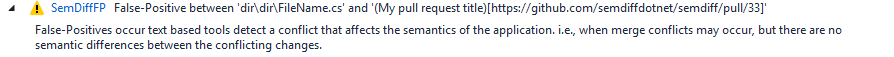
\includegraphics[width=\linewidth]{falsePositiveWarning.png}
	\caption*{Figure 12 - Capture of False-Positive Warning}
\end{figure}

\subsubsection{Future Work}
To finish this project, the warning system must be connected with the false-positive detection algorithm in order to get information on false-positives. The majority of the work will be will be in actually detecting the false-positives.

\subsection{Displaying False-Negatives Warnings in Error List}
SemDiff will display a warning in the “Error List” (at compile time) when a false-negative occurs between the semantics of the classes represented by the local files and the classes represented by the remote files retrieved from a pull request. This will require requirements 0 and 0 because the files and functionality to semantically diff will be needed.

We will show that a false-negative was detected.

We will show which classes are in conflict.

We will show which classes are in conflict.

We will provide a link to the pull request.

\subsubsection{Progress}
This warning system uses the same system as the false-positive warning system, therefore the system is not connected to the rest of the project, but currently exists and works.
Figure 13 shows the warnings in action. The format of this warning is as follows:
"False-Negatives for type '<<Type Name (Base Class)>>' between '(<<Title of Pull Request>>)[<<Link to Github>>]'"

\begin{figure}[h!]
	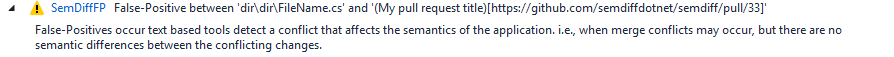
\includegraphics[width=\linewidth]{falsePositiveWarning.png}
	\caption*{Figure 12 - Capture of False-Positive Warning}
\end{figure}

\subsubsection{Future Work}
The same work as the false-positive warning system must be done. The only difference is the warning message will have a different warning code and body of the error.

\subsection{NuGet Package}
SemDiff will provide a NuGet package that can be installed to a VS project as an Analyzer.

\subsubsection{Progress}
Our project currently has the capability of producing a NuGet package. Figure 14 shows how our package will appear in the NuGet Package Manager.

\begin{figure}[h!]
	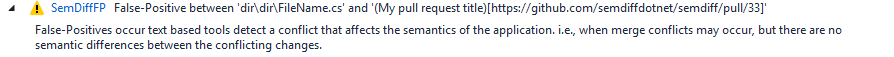
\includegraphics[width=\linewidth]{falsePositiveWarning.png}
	\caption*{Figure 12 - Capture of False-Positive Warning}
\end{figure}

\subsubsection{Future Work}
Our package could be improved by providing an icon for the package (this would replace the blue icon with white dots). After our package is installed extra things (our dependencies actually) show up in the analyzer section of the solution explorer, hopefully we will be able to resolve the issue. Currently we don’t think that it will be an issue, but affects the user experience.

\subsubsection{Problems}
Learning the nuspec configuration format was a significant barrier for this requirement. It seems as if few people have documented building a NuGet package for Roslyn Analyzers in particular. Because analyzers are very different from most packages, they require a different method for building the project and packaging the NuGet package. Luckily most of those problems have been resolved.

\subsection{Performance}
SemDiff will minimally impact VS performance.

Long term I/O bound work should use async-await (See MSDN Documentation).

Complex computation should be performed in a separate thread (See Task.Run())

We have implemented async functions in our request logic to improve the time to retrieve data from GitHub, however we have not done too much performance tuning yet as not all our code exists. We intent to make a table in our GitHub repo that will contain a table of compiling times (with and without our analyzer). We will use that to determine how much performance tuning will be necessary to fulfil this requirement.

\subsection{Informative Alerts}
Alerts will be informative

This requirement is largely redundant. The intent of this requirement was to contain the sub requirements from the 4 and 5, but was left behind (mostly by accident). It should be apparent that our alerts are informative because they contain all the information specified in their respective requirements.

\subsection{GitHub Project Hosting}
All source code, documentation, and issue tracking should be hosted publicly on GitHub.
GitHub wiki shall contain documentation for the project including a Getting Started guide, an API Guide with code examples, and motivational purpose of the project.

\subsubsection{Progress}
Currently our project source code is hosted on GitHub, we have also used been extensively using the issue tracking, pull requests, and milestone features built into GitHub. Currently we have 4 milestones, 10 open issues, 10 closed issues, and 13 closed pull requests. We also have our Wiki setup although it is light on content currently. Figure 15 shows the pages that we currently have.

\begin{figure}[h!]
	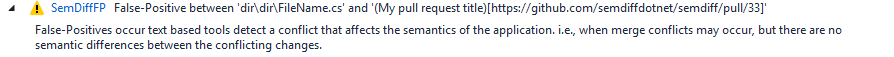
\includegraphics[width=\linewidth]{falsePositiveWarning.png}
	\caption*{Figure 12 - Capture of False-Positive Warning}
\end{figure}

\subsubsection{Future Work}
To complete this requirement, we will need to add a lot more content to our wiki, including an API Guide that details the parts of our application (including code examples). Especially our Getting Started Guide will need to be filled with high quality content. We have also added a performance section to detail how SemDiff effects the speed of compilation, we will need to measure the metrics and add that information to that page. In the future we may generate the API Guide using our XML documentation inside of the source code.

\subsubsection{Problems}
We had some difficulty in week 1 and 2 with Shawn not being able to commit to GitHub or make new issues, however that was resolved before it impacted our productivity. We also had some difficulty with using Git, the Git plugin for Visual Studio is not the easiest thing to use. This led to some code being pushed directly to the master branch. To resolve the issue (and submit the pull request like normal), we had to learn how to revert commits and revert merge commits. Before things were figured out we left a long string of revert commits and revert commits for revert commits. But the problem was resolved, and things have worked more smoothly since.

\subsection{MIT Licensing}
All outputs of the project should be open source and licensed with the MIT license.

A copy of the MIT license is available at the root of our GitHub repo and our final package includes a link to the MIT license. No more work should be needed to fulfil this requirement.

\subsection{Documentation in Code}
Source code will contain header comments on public classes, public interfaces, and public methods. Methods will only contain comments that help explain the function of obscure code.

Currently, the majority of our public items have good descriptions using the xml documentation, and there are no redundant comments in our code. Before SemDiff is complete we will have to do a review of the code to insure that all our public items have header comments and insure that our methods only contain relevant comments.

\subsection{Development Technology}
SemDiff will be built using C\# and the Roslyn API.

SemDiff is implemented in C\# and uses the Roslyn APIs to compare syntax trees and will use the APIs to help analyze for false-positives and false-negatives. In order to fulfil this requirement, we will need to continue to do develop in the same manner as we have been.

\section{Conclusion}
From the above information it is clear that we have an alpha level product. There is lots of work to do but we have a good start to having a well refined product at expo.

\section{Glossary}
.NET: Framework that provides the runtime and core libraries for C\# and other languages

AST: Abstract Syntax Tree is a parsed data structure that represents all of the tokens in source code.

C\#: Refers to C\# 6.0. Programming language that we are targeting. See https://goo.gl/y6A13i.

Diff: Tool that compares two versions of code to look for changes.

False-Positive: Error that occurs when one developer writes code that calls a function and creates a pull request while another developer creates a semantic change in the function that the previous developer depends on. This can change the actual functionality to differ from what is expected by the first developer even though the changes may merge (using text based tools) without warning. This can create subtle runtime bugs that can be difficult to detect. A false-positive is not caught by text-based diff software.

False-Negative: Errors that occur when one developer makes a non-semantic change (i.e., moves a function) and another makes a semantic change that conflicts (i.e., edits the contents of the function). When the pull request is merged (using text based tools), it will result in conflict even though semantic changes were only created by the latter developer.

GitHub: Website that provide version control, issue tracking, and documentation tools for software projects

NuGet Package: Open-source package manager for the Microsoft development platform. Provides the ability to produce and consume package in Visual Studio.

Roslyn: “Roslyn provides open-source C\# and Visual Basic compilers with rich code analysis APIs. It enables building code analysis tools with the same APIs that are used by Visual Studio.” – Roslyn Readme 
Semantics: Semantics of a program represent the executing behavior and the meaning/purpose of what is being executed. 
VS: Popular IDE for working with C\#, when used here it refers to Visual Studio 2015

See https://help.github.com/articles/github-glossary/ for git/GitHub related terminology

\begin{thebibliography}{1}

\bibitem{IEEEhowto:kopka}
H.~Kopka and P.~W. Daly, \emph{A Guide to \LaTeX}, 3rd~ed.\hskip 1em plus
  0.5em minus 0.4em\relax Harlow, England: Addison-Wesley, 1999.

\end{thebibliography}

\end{document}
